\documentclass[12pt, b5paper]{article}
\usepackage{ctex}

\usepackage{geometry}
\geometry{b5paper,left=2cm,right=1cm,top=2.5cm,bottom=2.5cm}
\usepackage{chemformula} %化学公式宏包
\usepackage[version=4]{mhchem} %化学公式宏包
\usepackage{siunitx} %数字，单位宏包
\sisetup{
	separate-uncertainty = true,
	inter-unit-product = \ensuremath{{}\cdot{}}
} %单位间加小圆点
\usepackage{tikz} %Tikz绘图包
\usetikzlibrary{cd}
\usetikzlibrary{chains}
\usetikzlibrary{arrows}
\usetikzlibrary{arrows.meta} %画箭头
\usetikzlibrary{commutative-diagrams} %交换图
\usetikzlibrary{positioning,automata}
\usepackage[all]{xy}
\usepackage{booktabs} %三线表
\usepackage{multirow} %合并单元格
\usepackage{makecell} %表格内强制换行
\usepackage{array}
\usepackage{booktabs} %控制表格行高
\usepackage{colortbl}  %彩色表格需要加载的宏包
\usepackage{amsmath}
\usepackage{unicode-math}
\usepackage{fontspec} %字体
\newcommand*{\cred}{\textcolor{red}}
\setmainfont{Times New Roman}
\setmathfont{XITS Math}
\setCJKmainfont{SimSun}[AutoFakeBold, AutoFakeSlant] 

\setlength{\parindent}{0pt} %无缩进
\usepackage{setspace}
\usepackage{fancyhdr} %设置页码
\usepackage{lastpage} %获取总页数
\pagestyle{fancy} %fancyhdr宏包新增的页面风格
\renewcommand\headrulewidth{0pt} %取消页眉中的装饰分割线
\fancyhf{}
\cfoot{\footnotesize 第 \thepage\ 页(共 \pageref{LastPage}页)}%当前页 of 总页数



\begin{document}


\begin{spacing}{1.625}

\centerline{{\huge \bf{河北农业大学课程考试试卷}}}

\centerline{\bf{\large 20\underline{24}年春（\quad ）/秋（\ \surd \ ）学期}}

{\bf{考试科目：\underline{\quad 化学反应工程 \quad} \hfill 姓名：\underline{ \qquad \qquad} \hfill 学号：\underline{ \qquad \qquad \qquad \qquad}}}

{\bf{学院：\underline{\quad 理工系\quad } \hfill 专业班级：\underline{\qquad \qquad \qquad \qquad} \hfill 卷别：\cred{B} \hfill 考核方式：\cred{开卷}}}

（注：考生务必将答案写在答题纸上，标清楚大小题号，写在本试卷上无效）

\bigskip


{\bf{一、简答题（共50分）}}

1. （10分）什么是半间歇操作？半间歇适用于什么场合？

\bigskip

2. （10分）液相平行反应：
\[
	\ch{A + B -> P} \qquad r_\mathrm{P} = k_1c_\mathrm{A}c_\mathrm{B}^{0.3} \ \mathrm{kmol\cdot m^{-3}\cdot min^{-1}}
\]
\[
	\ch{A + B -> Q} \qquad r_\mathrm{Q} = k_2c_\mathrm{A}^{0.5}c_\mathrm{B}^{1.3} \ \mathrm{kmol\cdot m^{-3}\cdot min^{-1}}
\]
Q为目标产物，请选择一种合适的反应器型式及加料方式。

\bigskip

3. （10分）绝热温升的物理意义是什么？如何计算间歇釜式反应器、连续釜式反应器、管式反应器的绝热温升？

\bigskip

4. （10分）内扩散有效因子的影响因素有什么？如何降低内扩散的影响？

\bigskip

5. （10分）下图为在连续釜和间歇釜中进行一级不可逆连串反应\ch{A ->[k1] P ->[k2] Q}的收率与转化率的比较。解释图像。
\begin{figure}[htpb]
    \centering
    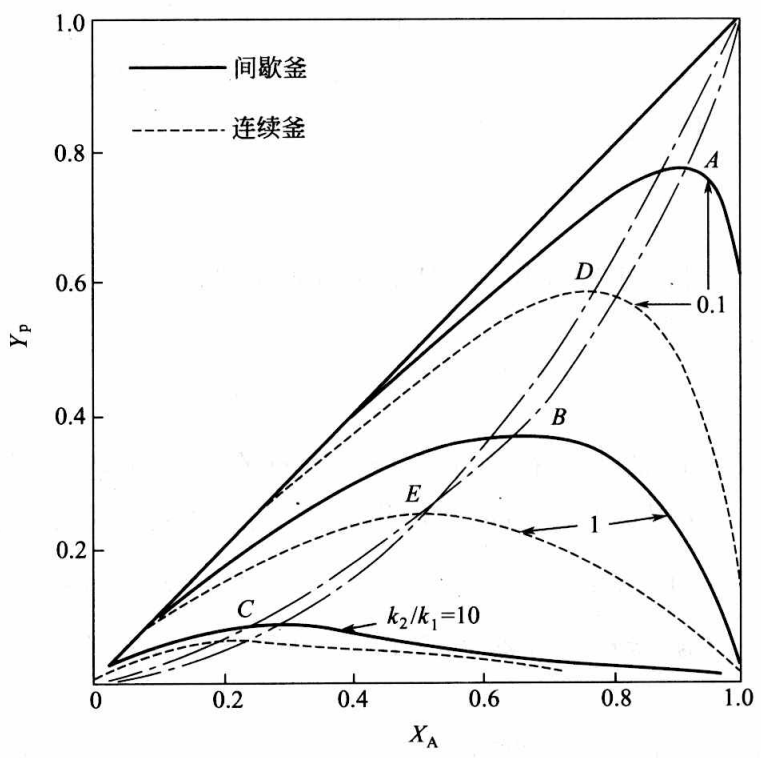
\includegraphics[width=.4\linewidth]{images/fig3.11}
\end{figure}

\newpage
{\bf{二、计算题(共50分)}}

1. (30分)等温下进行均相反应\ce{A -> B + C}，$r_\mathrm{A}=2.4c_\mathrm{A}$ (\si{mol.L^{-1}.h^{-1}})，每天生产B 20kmol，A的初始浓度为1mol/L，转化率为80\%。

(1) 反应在间歇操作的釜式反应器中进行，每批辅助时间为0.5 h，求反应体积。

(2) 反应在全混流反应器中进行，求反应体积。

(3) 反应在活塞流反应器中进行，求反应体积。

(4) 哪种反应器的反应体积最小？为什么？


\vspace{4em}
2. (20分) 乙烯直接水合制乙醇的初始反应速率符合一级反应动力学方程。在300℃，7.0 MPa时，其反应速率常数为0.09 s$^{-1}$。催化剂颗粒直径为5 mm，有效扩散系数$D_\mathrm{e} = 7.04\times 10^{-4}$ \si{cm^2/s}。试求催化剂颗粒的内部效率因子。

（注：$\tanh (x) = \frac{\mathrm{e}^x - \mathrm{e}^{-x}}{\mathrm{e}^x + \mathrm{e}^{-x}}$。当$x>3$时，$\tanh (x) = 1$）

\end{spacing}
\end{document}
